\documentclass[
../../Software_Engineering_Summary.tex,
]
{subfiles}

\externaldocument[ext:]{../../Software_Engineering_Summary.tex}
% Set Graphics Path, so pictures load correctly
\graphicspath{{../../}}

\begin{document}
\section{Software Architecture}
Software Architecture is concerned with how the software is designed and implemented. It is often a combination of design and implementation and is often defined in terms of dimensions. 

Software Architecture is a fast evolving and ever changing field. Some practices of the past are nowadays discouraged, while some others, which were once discouraged, are now encouraged.

\subsection{Architects and Developers Interoperability}
Architects and Developers work together closely. They give each other feedback and adapt to each others works. This is done iteratively, which promotes the evolution of the software.

\begin{defbox}
    [Architects]
    \begin{itemize}
        \item Extract the architecture characteristcs from requirements analysis
        \item Choose set of styles for software system
        \item Create the component structure
    \end{itemize}
\end{defbox}

\begin{defbox}
    [Developers]
    \begin{itemize}
        \item Design class structure for each component
        \item Design user interface
        \item Write and test source code
    \end{itemize}
\end{defbox}

\subsection{Dimensions}
\begin{defbox}
    [Architectural Characteristics]
    Concerned with how different characteristcs the software should fulfill.
    \begin{center}
        \begin{tabular}{|c|c|c|}
            \hline
            \rowcolor{codered!40}\textbf{Operational} & \textbf{Structural} & \textbf{Cross-Cutting}\\
            \hline
            Availability & Extensibility & Accessibility\\
            Scalability & Maintainability & Privacy\\
            Performance & Leveragibility & Security\\
            \dots & \dots & \dots\\
            \hline
        \end{tabular}
    \end{center}
\end{defbox}

\begin{defbox}
    [Architectural Style (Software System Structure)]
    Concerned with different layers of a software system are connected.

    \begin{center}
        \begin{tabular}{|c|}
            \hline
            \rowcolor{codered!40!white}\textbf{Presentation Layer}\\
            \hline
            \rowcolor{codeblue!40!white}\textbf{Business Layer}\\
            \hline
            \rowcolor{codegreen!40!white}\textbf{Persistence Layer}\\
            \hline
            \rowcolor{yellow!40!white}\textbf{Database Layer}\\
            \hline
        \end{tabular}
    \end{center}
\end{defbox}

\begin{defbox}
    [Decisions Concerning Architecture]
    Clarifies some questions before the architecture is implemented. For example:
    \begin{itemize}
        \item Which web framework?
        \item What are each layers responsibilities?
        \item How do layers communicate with each other?
        \item Which data formats should be used?
        \item \dots
    \end{itemize}
\end{defbox}

\begin{defbox}
    [Design Principles]
    Concerned with how the architecture should be implemented on a technical level. For example:
    \begin{itemize}
        \item NoSQL Databases are preferred
        \item Immutable data structures are preferred
        \item Asynchronous messaging between services when possible
        \item Avoid usage of caching in clients
        \item \dots
    \end{itemize}
\end{defbox}

\subsection{Architecture Characteristics}
\begin{itemize}
    \item Specifies non-domain design consideration: How to implement a given requirement
    \item Influences the structural design aspects: Requirements of specific architectural elements
    \item Critical that application performs as intended: Meets functional and non-functional requirements
\end{itemize}

\begin{defbox}
    [Operational Characteristics]
    \begin{itemize}
        \item \textbf{Availability:} When the system must be operational (specific times, continous, etc.)
        \item \textbf{Performance:} Response time, peak analysis, stress test, etc.
        \item \textbf{Scalability:} Functions with increased numbers of requests, users, etc. 
    \end{itemize}
\end{defbox}

\begin{defbox}
    [Structural Characteristics]
    \begin{itemize}
        \item Extensibility: Ability to add new features
        \item Maintainability: Ability to modify existing features
        \item Leveragibility: Ability to reuse existing features
        \item Localization: Support for different languages, currencies, units, etc.
        \item Configuration: Ability for user to configure the system to their needs via configuration interface
    \end{itemize}
\end{defbox}

\begin{defbox}
    [Cross-Cutting Characteristics]
    \begin{itemize}
        \item Accessibility: Usability for a lot of people, especially people with disabilities
        \item Privacy: User data inaccessible to unauthorized parties
        \item Security: Encryption of database, network traffic, authentication, authorization, resilience to attacks, etc.
    \end{itemize}
\end{defbox}

\subsection{Architectural Styles}
\begin{itemize}
    \item Help specify fundamental structure of a software system
    \item Impacts appearance of concrete software architectures
    \item Defines global properties:
    \begin{itemize}
        \item Interoperability of components
        \item Boundaries of subsystems
        \item etc.
    \end{itemize}
\end{itemize}
A software system can have multiple architectural styles.

An architectural style does almost always bring trade-offs. Being aware of them is important to choose the right one for your needs.

\subsection{Monolithic Architectural Styles}
\subsubsection{Layered Architectural Styles}
    \begin{center}
        \begin{tabular}{|c|c|c|}
            \hline
            \rowcolor{codered!40}\textbf{Operational} & \textbf{Structural} & \textbf{Cross-Cutting}\\
            \hline
            Availability & Extensibility & Accessibility\\
            Scalability & Maintainability & Privacy\\
            Performance & Leveragibility & Security\\
            \dots & \dots & \dots\\
            \hline
        \end{tabular}
    \end{center}

\begin{defbox}
    [Trade-Offs]
    \begin{minipage}
        [t]{0.5\textwidth}
        \centering
        \begin{itemize}
            \item[+] Simplicity
            \item[+] Cost
            \item[+] Reliability  
        \end{itemize}
    \end{minipage}
    \hfill
    \begin{minipage}
        [t]{0.5\textwidth}
        \centering
        \begin{itemize}
            \item[-] Elasticity and scalability
            \item[-] Performance (No parallelization)
            \item[-] Availability (Long startup time)
        \end{itemize}
    \end{minipage}  
\end{defbox}

Layered Architectures in general:
\begin{itemize}
    \item Technologically partitioned, not domain partitioned
    \item Works well for small to medium sized systems
    \item Serves as a starting point for larger systems, can be changed later
    \item Problem: Often created unconciously as it reflects the organisational structure of the company
\end{itemize}

\subsubsection{Pipes and Filters}
\begin{figure}
    [htp]
    \centering
    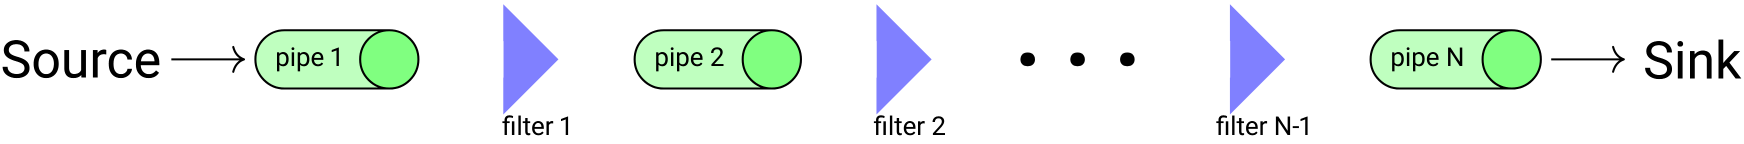
\includegraphics[width = 0.85\textwidth]{Pics/05/PipesAndFilters.png}
\end{figure}

\begin{defbox}
    [Pipes and Filters]
    \begin{itemize}
        \item Pipes:
        \begin{itemize}
            \item Unidirectional, point-to-point channels from data source to target
            \item Allow any data format, although smaller data formats are preferred for better performance
        \end{itemize}
        \item Filters:
        \begin{itemize}
            \item Self contained and independent from other filters
            \item Stateless, does not depend on past data and realizes exactly one task
        \end{itemize}
    \end{itemize}
\end{defbox}

\begin{defbox}
    [Different Types of Filters]
    \begin{itemize}
        \item Producer:
        \begin{itemize}
            \item Producer: Source of data
            \item Transformer:
            \begin{enumerate}
                \item Receives data from input channel
                \item Performs operations on the data
                \item Forwards result via output channel
            \end{enumerate}
            \item Consumer: Sink of data, Display output, written file, database, etc.
            \item Tester:
            \begin{enumerate}
                \item Receives data from input channel
                \item Tests whether data satisfies certain conditions
                \item Redirects data accordingly to different output channels
            \end{enumerate}
        \end{itemize}
    \end{itemize}
\end{defbox}

\begin{figure}
    [htp]
    \centering
    
\includegraphics[width = 0.85\textwidth]{Pics/05/PipesAndFiltersExample.png}
    \caption{Example of Pipes and Filters: Image Processing}
\end{figure}

\subsubsection{Model-View-Controller (MVC)}
\begin{figure}
    [htp]
    \centering
    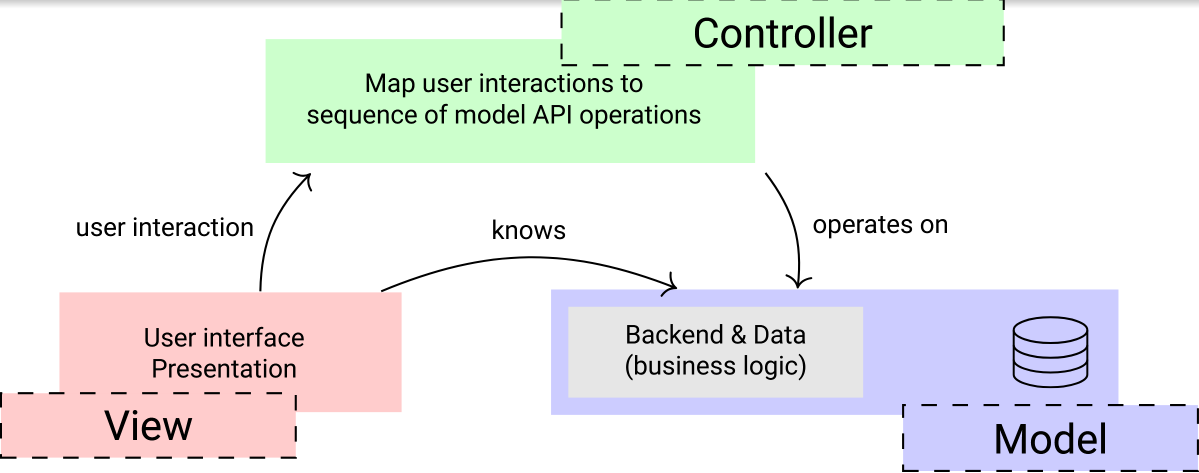
\includegraphics[width = 0.85\textwidth]{Pics/05/ModelViewController.png}
\end{figure}

\begin{defbox*}
    \begin{itemize}
        \item Seperates system into three parts:
        \item Model:
        \begin{itemize}
            \item Business logic and data storage
            \item Independent of input behaviour and output representation
        \end{itemize}
        \item View:
        \begin{itemize}
            \item Presentation of the model data to the user
            \begin{itemize}
                \item Data obtained from model
                \item Often more than one view
            \end{itemize}
        \end{itemize}
        \item Controller:
        \begin{itemize}
            \item Translates user interactions to operations on the model
            \item Each view has its own controller
            \item All interactions with the model are done via the controller
        \end{itemize}
        \item Controller and View are directly coupled with the model
        \item The model is independent of the controller and view
    \end{itemize}
\end{defbox*}

\begin{defbox}
    [Change Propagation Mechanism]
    \begin{itemize}
        \item Ensures consistency between the UI and the model
        \item Views register themselves at a model (Controllers too if behaviour depends on model state)
        \item Model notifies registered objects of changes
    \end{itemize}
\end{defbox}

\begin{defbox}
    [Trade-Offs]
    \begin{itemize}
        \item Updates all registered objects, even if they are not affected
        \item Increase in complexity due to seperate view and controller components without gaining much flexibility
        \item High dependency between view and controller
    \end{itemize}
\end{defbox}

MVC should be used when:
\begin{itemize}
    \item Application is interactive and:
    \item Number and kind of views are not fixed or unknown
    \item Display and application behaviour must reflect changed immediately
    \item Changing and porting the ui should not affect the applications core
\end{itemize}

\subsection{Distributed Architectural Styles}
\subsubsection{Service-Based}
Service-Based Architecture is a style of software architecture where the application is decomposed into service components that are independent of each other and are able to be provided separately. They can take different forms:

\begin{figure}
    [htp]
    \centering
    \begin{minipage}
        [t]{0.47\textwidth}
        \centering
        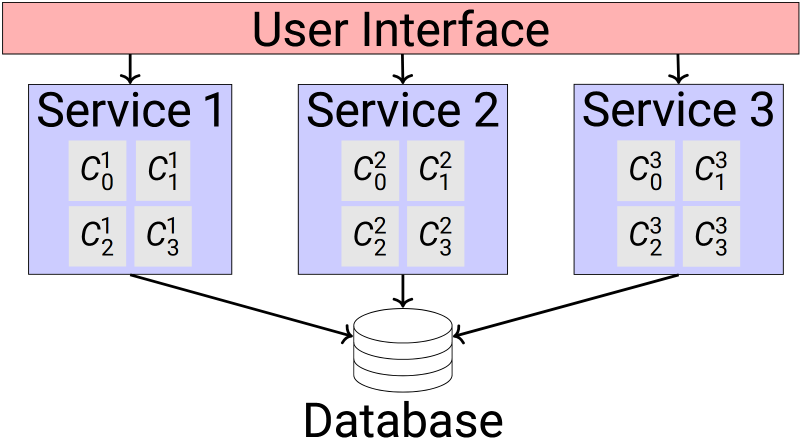
\includegraphics[width=0.95\textwidth]{Pics/05/ServiceBased1.png}
    \end{minipage}
    \hfill
    \begin{minipage}
        [t]{0.47\textwidth}
        \centering
        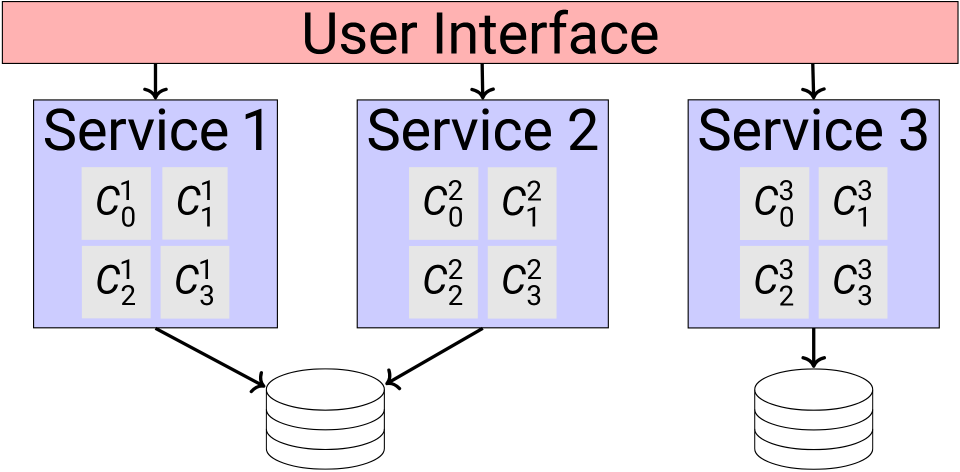
\includegraphics[width=0.95\textwidth]{Pics/05/ServiceBased3.png}
    \end{minipage}
    \newline
    \hspace{7pt}
    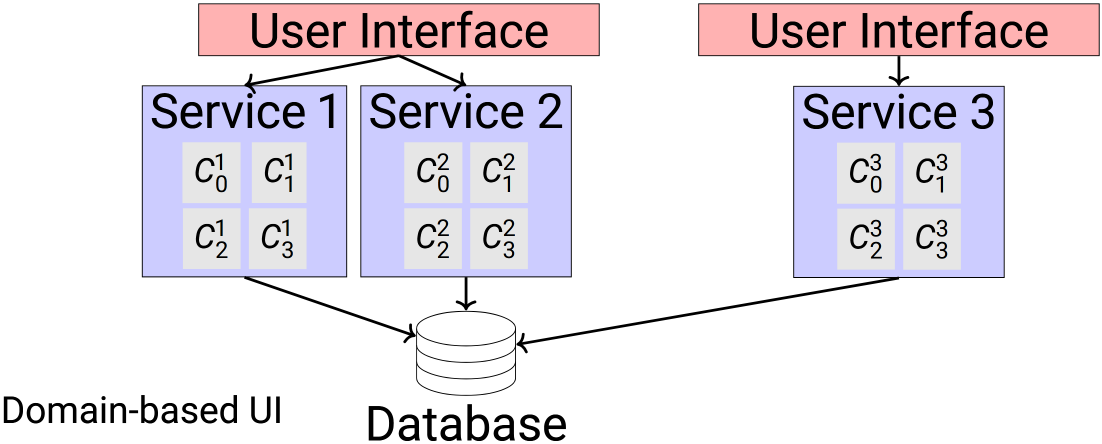
\includegraphics[width=0.6\textwidth]{Pics/05/ServiceBased2.png}
\end{figure}

In these examples access permissions must be defined. For example: One service might have read-only access to a database while another has write access.

More concrete this can look like this:
\begin{figure}
    [htp]
    \centering
    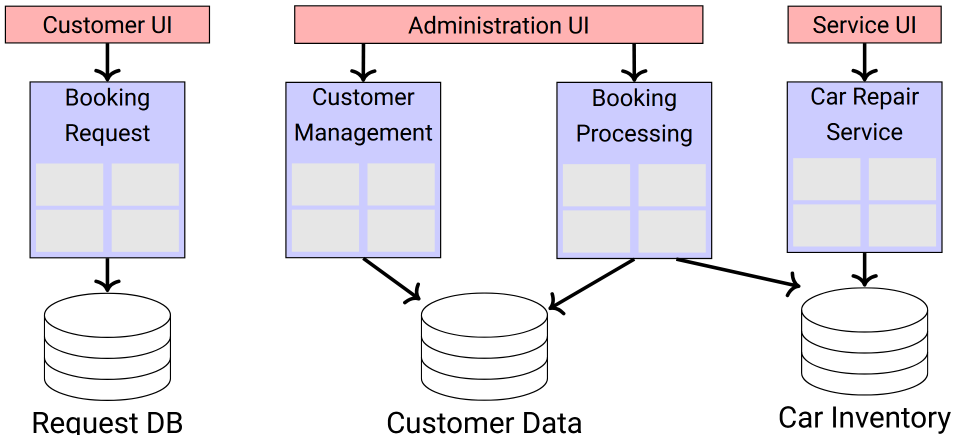
\includegraphics[width = 0.85\textwidth]{Pics/05/ServiceBasedExample.png}
\end{figure}

Choosing the right architecture style is tricky as it depends on many factors, such as the domain, the characteristcs, data architecture, organizational factors and the devolpment factors as a whole.

Therefore communication and documentation is very important.
\end{document}
